\begin{frame}{Introduction}
\begin{columns}[c]
    \begin{column}{0.55\textwidth}
        \centering
        \begin{tikzpicture}[scale=1, % scale down to fit column
          timeline/.style={draw=red, thick, -{Latex[length=2mm]}}, 
          event/.style={circle, draw=red, fill=red, minimum size=3pt, inner sep=0.6pt}, 
          label/.style={font=\scriptsize, align=left}
        ]
        % Text above the timeline
        \node[font=\small\bfseries, align=center] at (0,6.5) {Quantum Advantage};
        % Línia temporal vertical (arrow down)
        \draw[timeline] (0,6) -- (0,0);

        % Esdeveniments
        \node[event] at (0,5.5) {};
        \node[label, right=2pt] at (0,5.5) {1986\\R. Feynman};

        \node[event] at (0,3.5) {};
        \node[label, right=2pt] at (0,3.5) {May, 1994\\D. Simon};

        \node[event] at (0,1.5) {};
        \node[label, right=2pt] at (0,1.5) {November, 1994\\P. Shor};

        \end{tikzpicture}
    \end{column}
    \begin{column}{0.45\textwidth}
        \centering
            \vspace{-0.2cm}
            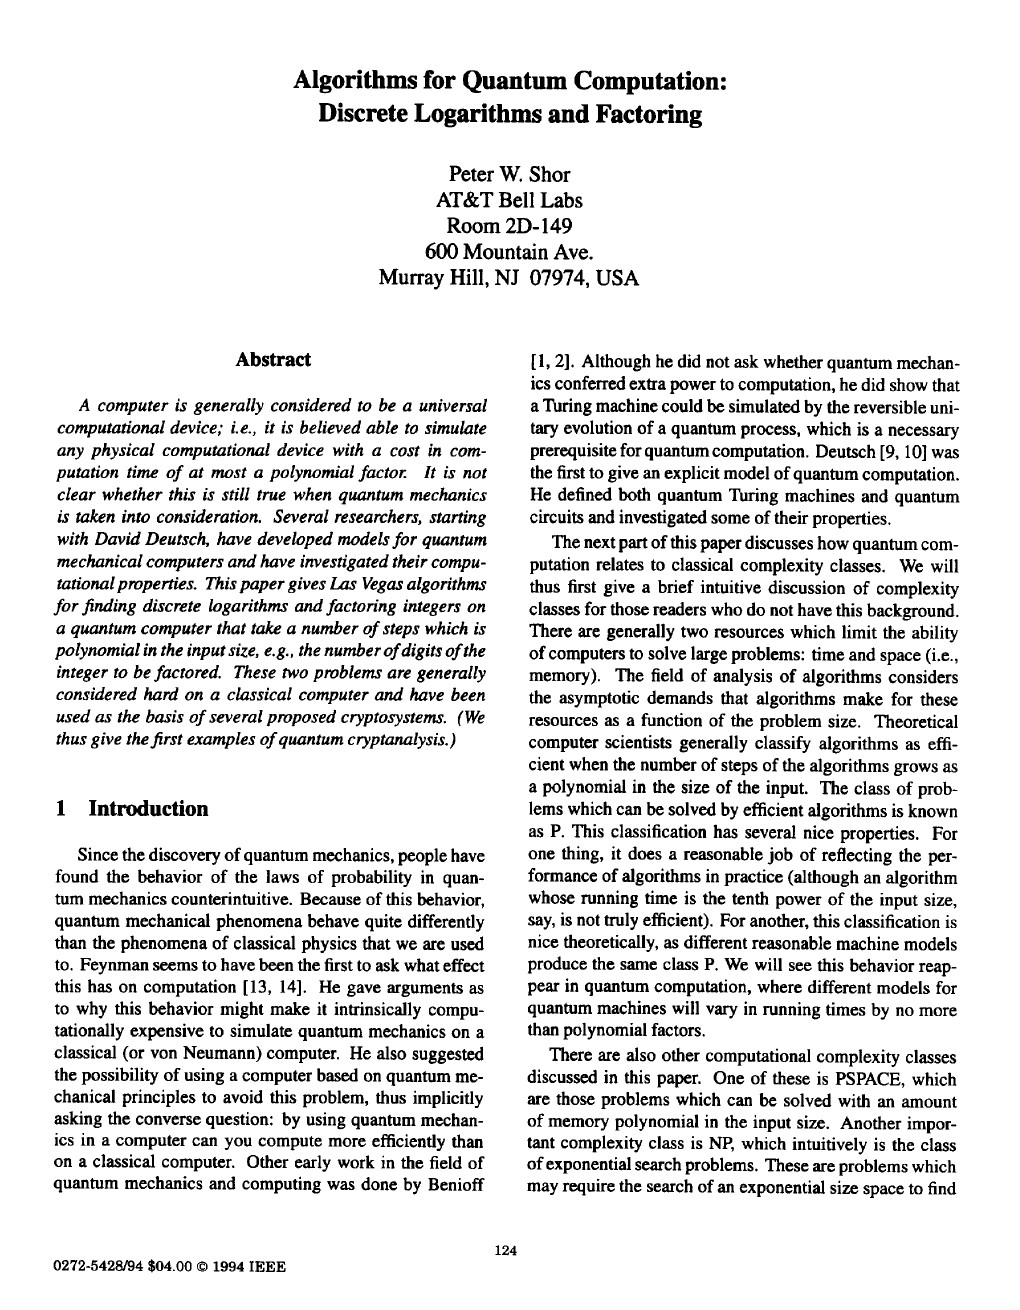
\includegraphics[width=0.9\linewidth, height=0.8
            \textheight, keepaspectratio]{Shor1994_pages-to-jpg-0001.jpg}
    \end{column}
\end{columns}
\end{frame}

